% \begin{figure*}[h!]
% \renewcommand{\thefigure}{S1}
%   \centering
%   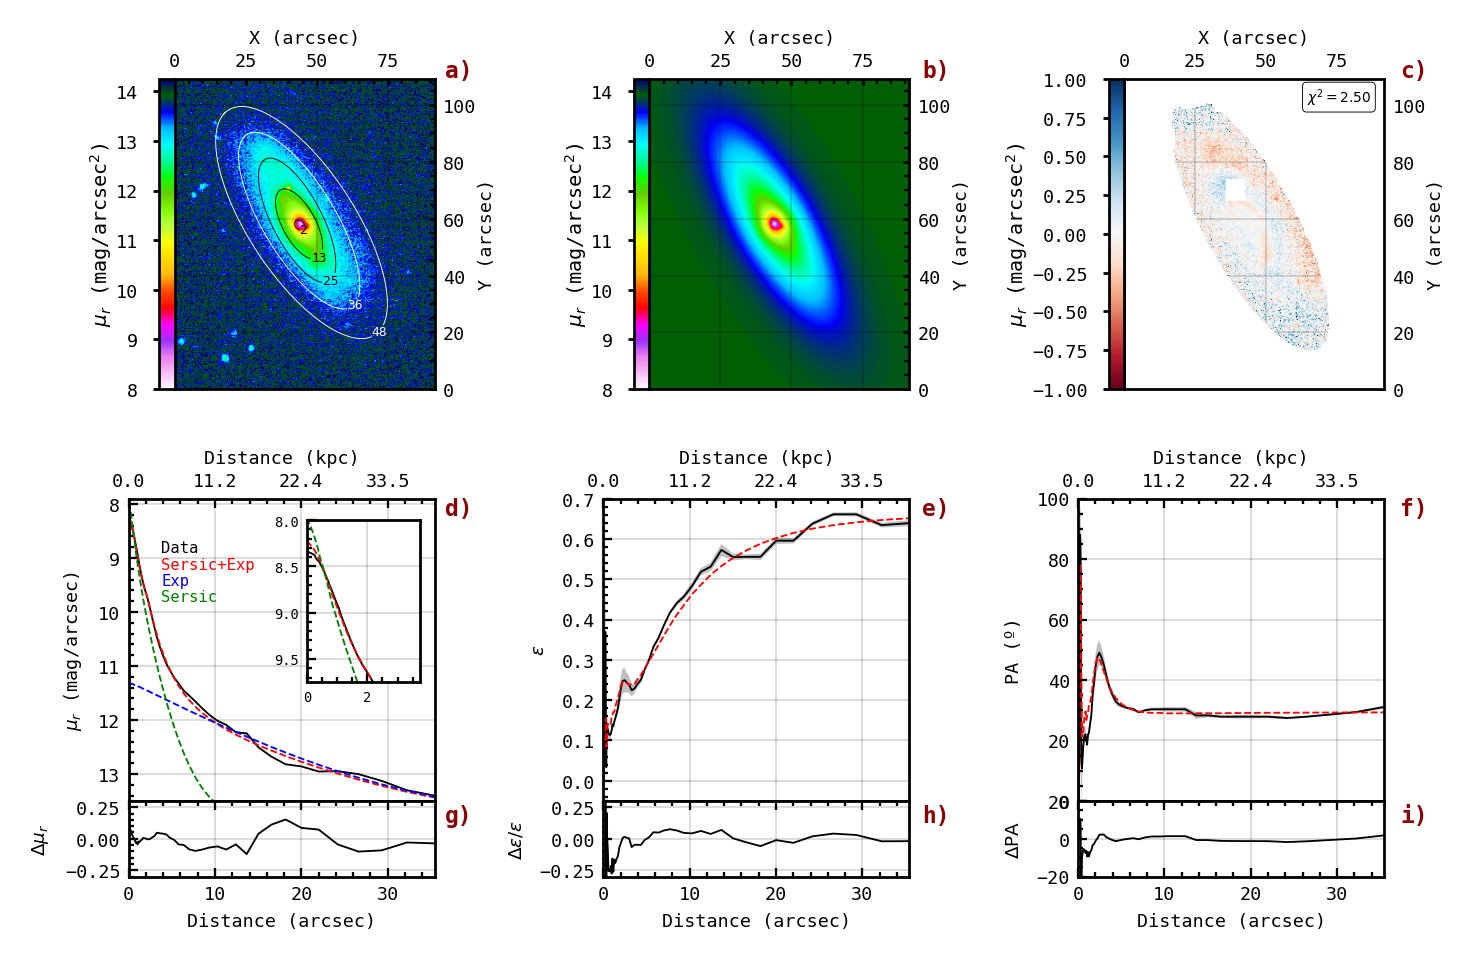
\includegraphics[width=\textwidth]{images/fit_sersic_exp_and_sersic_bump.png}
%   \caption{Photometric fitting of UGC09629 incorporating an exponential and a Sérsic model for the galaxy and an additional Sérsic model for the luminous bulb near the center of the galaxy, supplemented with elliptical isophote profile analysis. The reduced $\chi^2$ for the overall fit was 2.50. Image description is the same as Figure 2 in the main text.}
%   \label{fig:your_label}
% \end{figure*}


% \begin{figure*}[h!]
% \renewcommand{\thefigure}{S2}
%   \centering
%   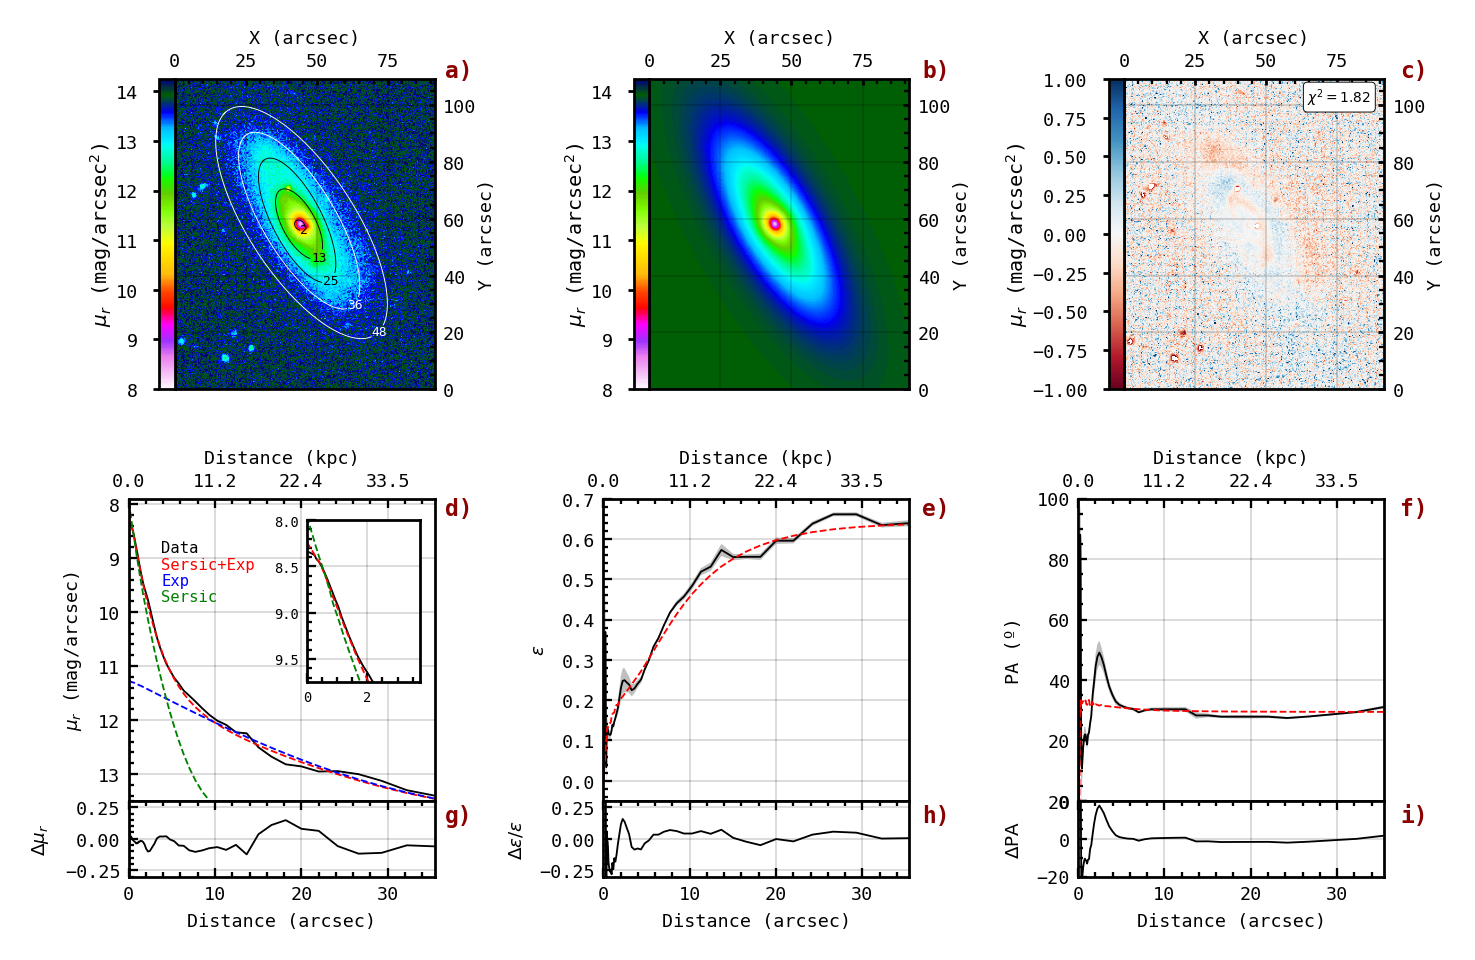
\includegraphics[width=\textwidth]{images/fit_sersic_exp_own_mask.png}
%   \caption{Photometric fitting of UGC09629 incorporating an exponential and a Sérsic model for the galaxy and using a customized \textit{ad hoc} mask, supplemented with elliptical isophote profile analysis. The reduced $\chi^2$ for the overall fit was 1.82. Image description is the same as Figure 2 in the main text.}
%   \label{fig:your_label}
% \end{figure*}